%%==================================================
%% chapter03.tex for SJTU Master Thesis
%% Encoding: UTF-8
%%==================================================

\chapter{实验与评估}
\label{chap:exp}

本章将描述本文系统设计的所有实验。
本文针对所设计的系统中每一个设计都进行了非项目参与人员的用户调研,分别是对三维菜单与操控手势的可行性评估,对单手操控、双手操控和辅助设计的易用性评估,
对空间设计基本操控的初步评估以及对用户进行具体建模要求的正式评估。
实验评估项目由用户的主观问答得分和被记录的客观时间次数参数组成。
从评估结果可见,混合现实眼镜下的三维界面、交互手段与徒手三维建模场景都具有一定的可行性与易用性。

\section{三维菜单与三维操控的可行性评估}
\label{sec:exp:feasibility}
首先,针对混合现实眼镜下的手势交互和菜单设计进行可行性评估。
\subsection{实验介绍}
开始,我们先给五位实验者(最小年龄 22 岁,最大年龄 25 岁,平均 23.4岁)简单介绍了本文系统,并展示了基本操控。实验者在此之前对该系统并无了解,也从未接触过 Oculus VR和 Leap Motion。然后开始训练,训练分为以下几步:
\begin{enumerate}
\item 使用菜单手势调用手掌召唤式菜单创建物体
\item 使用目标跟踪式菜单旋转物体
\item 使用屏幕固定式菜单放缩物体
\end{enumerate}

训练过后,实验者对本文系统有了初步的了解,开始正式实验任务。共有三个实验,实验步骤一致,但分别采用三种不同的菜单(手掌召唤式菜单、目标跟踪式菜单和屏幕固定式菜单)。实验步骤如下:

\begin{enumerate}
\item 在不同位置分别创建一个茶壶和一个茶杯
\item 使用单手操控将茶壶放置到茶杯的附近,呈现倾倒的状态
\item 使用双手操控将茶杯杯口向上
\item 拷贝这套茶具
\end{enumerate}

统计所得训练时间从 6 到 11 分钟不等,而完成三个实验总共需要 20 分钟左右。实验结束后,每个实验者都需完成一份调查问卷。

\subsection{可行性实验结果与分析}
\label{subsec:exp:feasibility}

\begin{figure}[!htp]
  \centering
  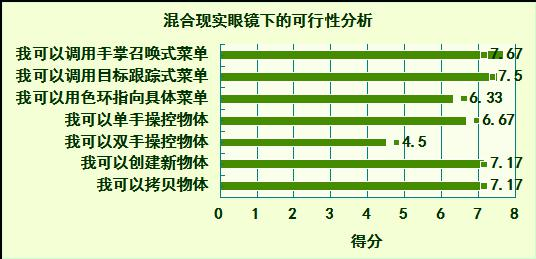
\includegraphics[width=0.8\textwidth]{chap6/eva-feasibility}
  \bicaption[fig:feasibility]{三维菜单与三维操控的可行性分析问卷}{三维菜单与三维操控的可行性分析问卷}{Fig.}{The feasibility questionnaire of 3D menus and 3D manipulation}
\end{figure}

所有的实验参与者都完成了训练,只有一个人在第四项实验任务中失败了。实验过程中我们发现参与者在操控方面都碰到了困难,一方面是从未使用过 Leap Motion,无法十分熟练地使用 Leap Motion,另一方面当物体没有按照参与者的预料变化时,参与者不知道应该如何处理,关于加强 Leap Motion 的操控方面,训练和更多的系统提示都是必要的。
这也就是后来在\ref{sec:interaction:skeleton}节中提到的骨骼小球增加的原因。

根据大家的问卷调查,我们得到了如图\ref{fig:feasibility}所示的可行性结果分析。参与者对所有项目进行打分,0 分为最低分表示最不认同,10 分为最高分表示最为认同。

首先评估本文系统设计的三种菜单(手掌召唤式菜单、物体跟踪式菜单和屏幕固定式菜单)。虽然三类菜单的得分互相间略有差异,但与操控物体类的得分相比都属偏高,说明触发菜单指令比操控物体更容易。有时由于过于灵敏,用户可能无意中做出菜单手势触发了菜单。而这个过于触发的误操作也就是\ref{sec:interaction:head}节提到的头部约束设定的来源。

其次评估选择操作。大多数参与者都表示可行,只有一个参与者遇到了困扰。其在实验中带着色环对物体进行操控时,物体没有随着手的变化而变化,因为带着色环是不能对物体进行操控操作的。当用户理解了本文系统在选择物体和操控物体的状态切换原则后,就消除了困惑。此外,由于选择菜单后,菜单消失的同时,菜单操作区域和物体操作区域可能重叠,导致实验者无意中选中物体。同时,有参与者提出,如果能在选中菜单后有更明显的状态提示,会更了解当前系统的情况。也是因此设计了\ref{fig:interaction:board}节提到的顶置提示板。

最后是操控类评估,单手操控物体的得分远大于双手操控。
原因有二,其一是单手操控的设计接近触摸屏的操作,参与者很快就熟悉了起来,而且表示不用一直拿着手机或者平板感觉轻松不少;
其二是双手操控物体时,常常因为距离或者角度的原因超过了 Leap Motion 的接收范围,以至于无法成功操作。此外,无论是单手还是双手操控,参与者都表示很难进行特别精细的操作,诸如旋转 90°,放大成原来的 2 倍等。

\section{三种菜单的偏好布局分析}

\subsection{实验介绍}
本次实验共有两个部分,一则比较不同的布局,一则比较批处理操作时大家喜好是否会有变化。实验邀请了 10 位志愿者,其中 8 位男生,2 位女生,实验任务介绍如下:
\begin{enumerate}
\item 实验者通过目标物系列菜单进行虚拟物体创建并缩放。目标物系列菜单为目标跟踪式菜单和屏幕固定式菜单,而在这项任务完成后对二者进行选择。
\label{exp:object-series}
\item 实验者使用完成实验\ref{exp:object-series}后选择的目标物系列菜单和手掌召唤式菜单分别对三个物体进行拷贝并将他们旋转至面朝右方,值得注意的是这里的具体操作流程并不一样也导致了之后实验的评估。
\label{exp:batch}

\subsection{三种菜单布局的喜好分析}
\end{enumerate}
\begin{figure}[!htp]
  \centering
  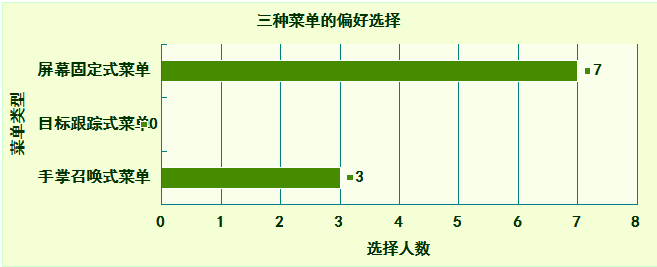
\includegraphics[width=0.8\textwidth]{chap6/preference}
  \hspace{1cm}
  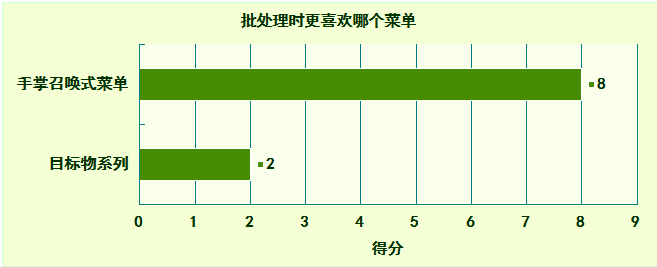
\includegraphics[width=0.8\textwidth]{chap6/batch}
  \bicaption[fig:preferenceMenu]{三种菜单的偏好选择}{三种菜单的偏好选择}{Fig.}{Preference on three types of menus}
\end{figure}

本次实验的目的是为了分析三种布局的菜单在用户心中的使用偏好。
并且当任务内容发生变化时,对三种类型的菜单选择是否会有变化。

图\ref{fig:preferenceMenu}显示没有用户喜欢目标跟踪式菜单。手掌召唤式菜单的特点是永远出现在手中,随掌而动;屏幕固定式菜单的特点是永远出现在屏幕中央,大而明晰;而对于目标跟踪式菜单,虽然从语义上紧跟目标物非常合理,但由于Oculus VR目前的像素以及菜单的逻辑设定会随目标物的朝向与大小而变,导致观察菜单的难度提升,这些都是影响因素。

同时选择屏幕固定式菜单和手掌召唤式菜单的人数中,一部分实验者倾向先确定目标物,于是他们偏好屏幕固定式菜单而另一部分实验者倾向先确定操作于是他们偏好手掌召唤式菜单。
接着在批处理(即实验\ref{exp:batch}中,大部分实验者都选择了手掌召唤式菜单,因为选择该菜单可以减少完成实验任务的步骤并且每个被操作的物体都可以互相保持一致的角度,使整个任务完成的质量更好。

\section{辅助设计与单手、双手操控的易用性评估}
\label{sec:exp:usability}

为了验证新增的几项修改是否有效,我们针对改进版的系统进行了更加正式的易用性评估。评估了如下内容:

\begin{enumerate}
\item 本文系统的总体使用感受
\item 提示板、手势可视化以及结合头部的手势设计这几方面的易用性
\item 单双手操控的比较和当前系统对精确操控的支持度
\end{enumerate}

\subsection{实验介绍}
同样从系统介绍开始,展示了系统的基本操控方法后,首先开始了训练步骤:
\begin{enumerate}
\item 使用 Leap Motion 训练菜单手势和操控手势
\item 启用顶置提示板,用手掌召唤式菜单创建物体
\item 启用骨骼小球,用目标跟踪式菜单对物体进行单手旋转
\item 启用头部约束,用屏幕固定式菜单对物体进行双手操控
\end{enumerate}

训练部分完成后,用户对新增的几种修改都有了大致了解,之后便是正式的实验任务,步骤如下:
\begin{enumerate}
\item 用手掌召唤式菜单创建茶壶和茶杯,启用头部约束和关闭各一次
\item 用目标跟踪式菜单单手操控茶壶,使之呈倾倒状,启用骨骼小球和关闭各一次
\item 用屏幕固定式菜单拷贝茶壶和茶杯,启用提示板和关闭各一次
\item 指定参考茶壶 A 和茶壶 B、 C,使用单手操控将茶壶 B 调整到与参考茶壶 A 大小朝向一致,再使用双手操控将茶壶 C 同样调整一遍
\label{item:uniandbi}
\end{enumerate}

整个实验过程中对每个提示启用与否的操控都有计时,用户完成实验后进行问卷填写。

\subsection{用户的总体使用感受}

首先,用户对混合现实眼镜有较大的兴趣,觉得直接能看到增强现实的场景,而不用通过屏幕,非常地直观,在满分 10 分的总体易用性评估中获得7.5 分。
并且对表示绑定在手上的菜单感觉新奇,仿佛自身的功能得到了增强。然而当前制作的增强现实眼镜仍然不够轻便,
且 OculusVR目前像素较低,几乎所有用户都在实验完成后表示头有些重,眼睛有些不适。

其次,用户对于不用佩戴沉重设备的近乎裸手
交互也表达了支持的态度,单手操控很顺畅就像空
中有一个触摸屏,双手操控效果也很令人激动只是
不够灵敏还需要再改进。

\begin{figure}[!htp]
  \centering
  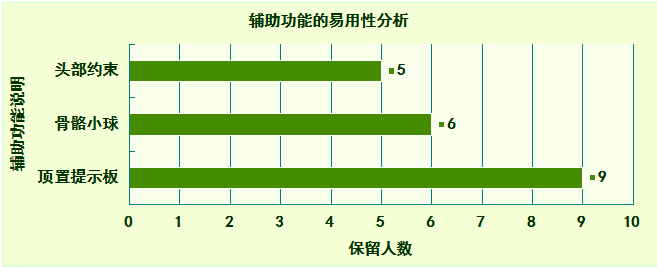
\includegraphics[width=0.8\textwidth]{chap6/fuzhu}
  %\hspace{1cm}
  %\includegraphics[width=0.3\textwidth]{chap6/testpng}
  \bicaption[fig:exp:usability]{辅助功能的易用性分析}{辅助功能的易用性分析}{Fig.}{The usability of the design for assistance}
\end{figure}

图\ref{fig:exp:usability}显示了改进版系统的易用性分析,数值表示参与实验的 10 人中愿意保留各项改进的人数。

\subsection{顶置提示板的易用性分析}
图\ref{fig:exp:usability}显示了用户对是否愿意保留提示板的看法,只有 1 名参与者表示无需提示板,感觉提示板的出现显得整个增强现实界面有点冗余,其他 9 名
参与者都支持这个新的补充。
根据表\ref{table:exp:skeleton}中记录的时间,实验任务 3 中实验者在打开提示板和关闭提示板的两种情况下,完成任务的时间基本一致。
虽然提示板没有在完成任务的效率上有明显提升,但在心理上给了用户更多的支持,值得保留。

此外,有 1 名实验者表示提示板的位置过高,注意力很难集中到视野的边缘处,关于提示板的安置位置或者变化时机,还可以做更多的改进。

\subsection{手势可视化之骨骼小球的易用性分析}

\begin{table}[!hpb]
  \centering
  \bicaption[table:exp:skeleton]{开启或关闭辅助功能的各项平均时间统计}{开启或关闭辅助功能的各项平均时间统计}{Table}{Average time consumption on enabling or disabling the assistance}
  \begin{tabular}{@{}cccc@{}} \toprule
    实验内容 & 实验1/秒 & 实验2/秒 & 实验3/秒 \\
	\midrule
    修改内容 & 头部约束 & 骨骼小球 & 顶置提示板 \\
    启动修改完成的平均时间 & 82 & 44 & 70 \\
    关闭修改完成的平均时间 & 143 & 70 & 85 \\
	\bottomrule
  \end{tabular}
\end{table}

图\ref{fig:exp:usability}显示了大家对是否愿意保留骨骼小球的看法。
多数实验者表示骨骼小球的提示是有用的,可以知道目前自己的手势是否被检测,检测的形态是什么样子,以此来调整自己的手势更好地进行操控任务。
而反对意见表示,有时候由于手势角度的原因 Leap Motion 检测到的手势比较混乱,于是整个场景就会被混乱的骨架所干扰,影响操控的效率。
1名实验者提议可以将手势骨架转化成两种文字提醒,一种提醒手势在Leap Motion检测区域内,另一种提醒超出范围以外即可。 
从表\ref{table:exp:skeleton} 的统计结果来说,启用骨骼小球在一定程度上对操控性能有所提升,值得保留。

\subsection{单手操控与双手操控的对比}
\begin{figure}[!htp]
  \centering
  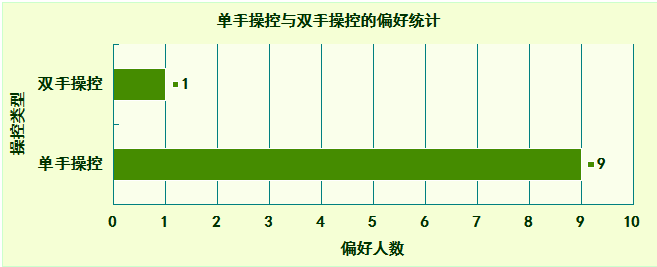
\includegraphics[width=0.8\textwidth]{chap6/univsbi}
  \bicaption[fig:exp:univsbi]{单手操控与双手操控的偏好统计}{单手操控与双手操控的偏好统计}{Fig.}{Preference on unimanual interaction and bimanual interaction}
\end{figure}

实验\ref{item:uniandbi}中,参与者使用单手操控和双手操控的方法对物体进行了控制。
从图\ref{fig:exp:univsbi} 中可以看到,绝大部分用户喜欢单手操控,原因与\ref{subsec:exp:feasibility}节分析的一致。
还有用户提到,经常需要切换具体指令如单手平移等,有些不便。
而选择双手操控的 1名用户是任务完成中最快最好的,一方面无需不停地进行状态切换,一方面双手的操控和现实更为接近,十分直观。
然而在实验\ref{item:uniandbi}中,所有参与者都表示要使被操控的物体和参考物体在姿态上完全相似,非常困难,难以精细地对物体进行旋转,无论是单手操控还是双手操控,原因是操控中手部和头部的轻微移动会影响操控的效果,这也是本文系统目前的不足。

\section{空间设计的基本操控评估}
\label{sec:exp:pilot}
本次实验针对本文工作中的空间设计部分,进行混合现实眼镜下的基本操控评估。

\subsection{实验介绍}
本次实验的环境就在实验室中,完全日常的环境配备,无需特殊的调整。
参与人员由14个研究生和1个本科生组成。其中10名男生,5名女生,年龄从20到25岁不等,平均为22.8岁,标准差为1.42。
所有人的惯用手都是右手,其中9名实验者曾使用过虚拟现实或者增强现实的设备,所有人都没有参与到本文系统的设计实现中。
基本操控评估包括手势和基本功能的测试,以下为实验步骤:
\begin{enumerate}
\item 使用右手自然张开五指配置初始化的自由虚拟网格平面
\item 在指定的四个紫色点上绘制控制点
\label{exp:cp}
\item 使用切换工具的手势将旋转工具切换为放缩工具
\item 选择旋转工具中的某具体坐标轴
\end{enumerate}

以下为评估标准,一共是三项:
\begin{enumerate}
\item 执行时间(Execute Time/ET) \hfill \\
实验者在每个单项任务上所耗费的时间
\item 误操作率(Rate of Misoperation/RM) \hfill \\
用错误的次数比上全部的尝试次数。如当用户想要旋转虚拟网格平面时,错误地变换了控制工具等。这就视为一次误操作。
\item 准确率(Rate of Accuracy/RA) \hfill \\
用正确的次数比上总共尝试的次数。如要求实验者选中指定的目标物,如果指到了则视为一次正确的操作。
\end{enumerate}

\subsection{基本操控实验结果分析}

\begin{figure}[!htp]
  \centering
  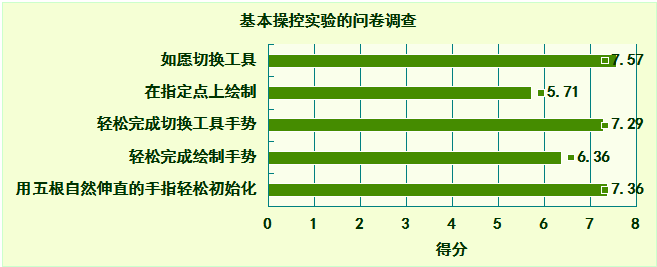
\includegraphics[width=0.8\textwidth]{chap6/eva-question}
  \bicaption[fig:spcItrc:basic]{基本操控实验的问卷调查}{基本操控实验的问卷调查}{Fig.}{The questionnaire of pilot experiment}
\end{figure}

在所有的实验过程中,只有1名实验者没有完成所有的任务,究其原因因为Leap Motion设备始终无法正确捕获他的手指类别,而这一点在应用设计中是有具体对应的。
另外14个参与者都成功完成实验。
对于空间设计中的基本操控感受,每个实验者都完成了一份主管的问卷调查,显示在图\ref{fig:spcItrc:basic}中,分值从0浮动到10,分数越高越表示赞同。

%\begin{figure}[!htp]
  %\centering
  %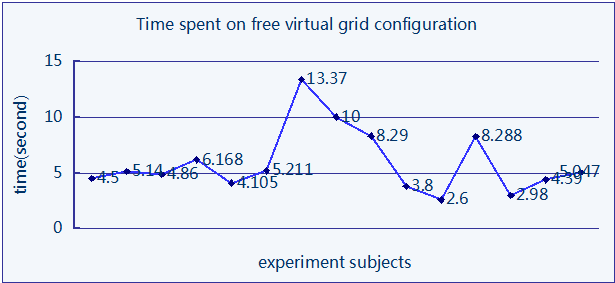
\includegraphics[width=0.6\textwidth]{chap6/eva-fvg-call}
  %\bicaption[fig:spcItrc:initial]{设定初始自由虚拟网格平面耗时}{设定初始自由虚拟网格平面耗时}{Fig.}{Time consumption on initializing free virtual grid}
%\end{figure}

如表\ref{table:exp:initial}所示,整个实验花去用户2秒到13秒不等的时间来进行初始网格平面的调整(ET)。
之所以有部分实验者花费超过十秒的时间来设置初始设定是为了在之后的实验中获得更好的体验。
尤其当实验者能够长时间进行放置自由虚拟网格平面的操作时,也就是表明实验者对这一手势的熟悉。
没有任何一名实验者在这一任务上失败,并且从图\ref{fig:spcItrc:basic}的问卷调查中也可以看到对这一动作大家觉得很轻松。

\begin{table}[!hpb]
  \centering
  \bicaption[table:exp:initial]{完成易用性实验的平均时间统计}{完成易用性实验的平均时间统计}{Table}{Average time consumption for feasibility experiment}
  \begin{tabular}{@{}ccc@{}} \toprule
    实验者编号 & 初始化耗时/秒 & 切换工具耗时/秒\\
	\midrule
    1 & 4.5 & 4.9\\
	2 & 5.14 & 3.8\\
	3 & 4.86 & 6\\
	4 & 6.168 & 1.7\\
	5 & 4.105 & 1.6\\
	6 & 5.211 & 3.628\\
	7 & 10 & 2.21\\
	8 & 8.29 & 1.737\\
	9 & 3.8 & 1.838\\
	10 & 2.6 & 2.479\\
	11 & 8.288 & 10\\
	12 & 2.98 & 2.145\\
	13 & 4.39 & 2.628\\
	14 & 5.047 & 2.729\\
	平均值 & 5.384 & 3.386\\
	标准差 & 2.125 & 2.303\\
	\bottomrule
	%&5.14&4.86&6.168\\
	%切换工具耗时 & 4.9 & 3.8 & 6 & 1.7 \\
	  %实验单位 & 实验者5 & 实验者6 & 实验者7 & 实验者8 \\
	  %初始化耗时 &4.105&5.211&10&8.29\\
	  %切换工具耗时  & 1.6& 3.638 & 2.21 & 1.737 \\
	  %实验单位 & 实验者9 & 实验者10& 实验者11 & 实验者12 \\
	  %初始化耗时&3.8&2.6&8.288&2.98\\
	  %切换工具耗时 & 1.838 & 2.479& 10 & 2.145 \\
	  %实验单位 & 实验者13 & 实验者14 & 平均值&标准差\\
	  %初始化耗时&4.39&5.047&5.384214286 & 2.125342223\\
	  %切换工具耗时& 2.628 & 2.729 & 3.386 & 2.303924812\\
	  %\bottomrule
  \end{tabular}
\end{table}

%\begin{figure}[!htp]
  %\centering
  %\begin{subfigure}[b]{0.3\textwidth}
                %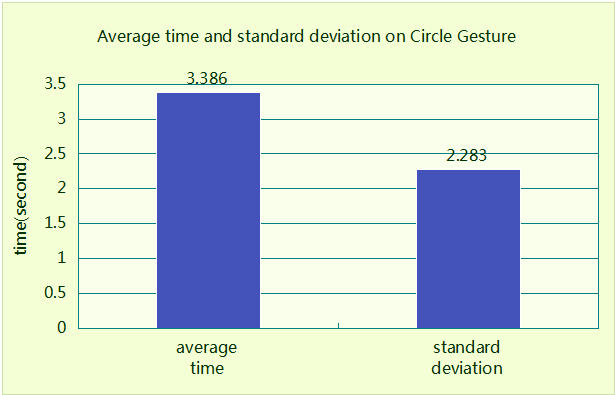
\includegraphics[width=\textwidth]{chap6/eva-fvg-circle}
                %\bicaption[fig:spcItrc:circle]{切换工具手势耗时}{切换工具手势耗时}{Fig.}{Time consumption on circle gesture}
  %\end{subfigure}
  %\hspace{1in}
  %\begin{subfigure}[b]{0.3\textwidth}
                %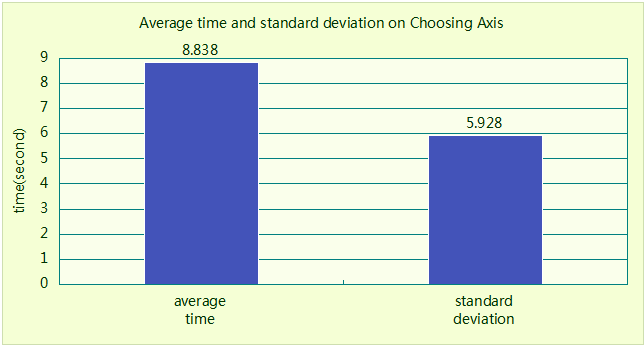
\includegraphics[width=\textwidth]{chap6/eva-fvg-choose-axis}
                %\bicaption[fig:spcItrc:axes]{选择坐标轴耗时}{选择坐标轴耗时}{Fig.}{Time consumption on choosing axes}
  %\end{subfigure}
  %\bicaption[fig:spcItrc:time]{切换工具手势和选择坐标轴的耗时}{切换工具手势和选择坐标轴的耗时}{Fig.}{Time consumption on circle gesture and choosing axes}
%\end{figure}

%\begin{figure}[!htp]
  %\centering
  %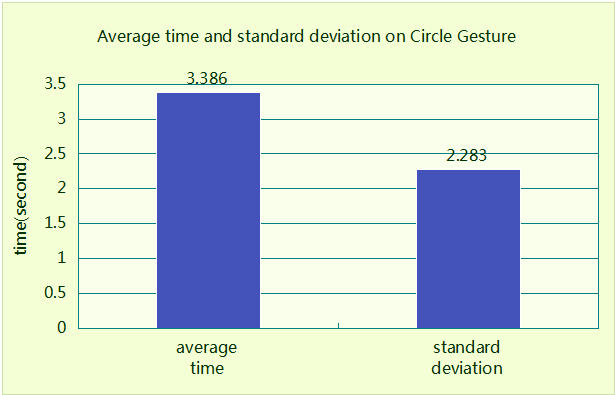
\includegraphics[width=0.4\textwidth]{chap6/eva-fvg-circle}
  %\hspace{1cm}
  %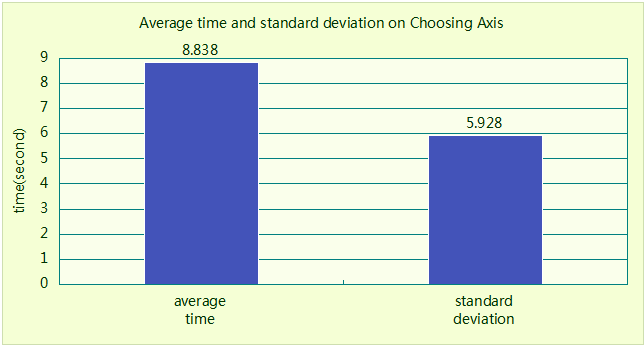
\includegraphics[width=0.4\textwidth]{chap6/eva-fvg-choose-axis}
  %\bicaption[fig:spcItrc:time]{切换工具手势和选择坐标轴的耗时}{切换工具手势和选择坐标轴的耗时}{Fig.}{Time consumption on circle gesture and choosing axes}
%\end{figure}

如表\ref{table:exp:initial}所示,实验者通常需要少于3秒的时间来完成切换工具的手势(ET)。
而在整个实验进行中,当实验者执行其他操作时并没有出现意外地切换工具的情况发生(RM)。
如图\ref{fig:spcItrc:axes}所示,实验者要花费更多的时间在选择坐标轴上(ET),但同样发现图\ref{fig:spcItrc:axes}中的标准差亦是很大,可见不同的实验者所需的时间差别很大,进一步了解到这同样受当前坐标轴的位置和要选择的坐标轴是哪一个有关。
当进行\ref{sec:exp:model}节的建模实验时,我们并没有发现实验者对于选择特定的坐标轴来进行旋转操作有任何困难。
除此之外,我们同样可以从图\ref{fig:spcItrc:basic}中获悉实验者在切换工具这一项上给了高分,可见这一建模方法在一定程度上还是轻松易学的。
\begin{figure}[!htp]
  \centering
  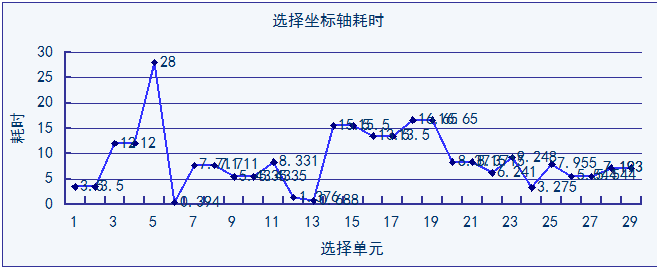
\includegraphics[width=0.9\textwidth]{chap6/selectaxes}
  \bicaption[fig:spcItrc:axes]{选择坐标轴耗时}{选择坐标轴耗时}{Fig.}{Time consumption on choosing axes}
\end{figure}

如图\ref{fig:spcItrc:selcp}所示,几乎所有的实验者都能在自由虚拟网格平面上选定给定的四个控制点(RA),其中两名实验者没有成功选择因为他们没有理解必须在几乎和自由虚拟网格平面同一个平面上进行控制点的绘制,也就是工作空间的概念。
有时实验者的手指在该网格平面的正上方,虽然看起来正指在某个控制点上,但其实尚有距离。反过来思考着一点,实验者便可以通过抬高或降低自己的手的平面来防止自己无意中对控制点的选择,减少误操作。

\begin{figure}[!htp]
  \centering
  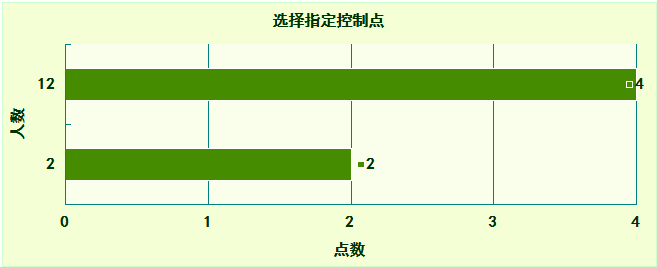
\includegraphics[width=0.8\textwidth]{chap6/eva-select-points}
  \bicaption[fig:spcItrc:selcp]{选择指定控制点}{选择指定控制点}{Fig.}{Choosing specific points}
\end{figure}

在基本操控实验之后,实验者对与本文系统设计的空间设计也有了一定了解。整个实验的介绍约莫十分钟而整个基本操控实验耗时也接近十分钟,部分实验者对操控旋转工具非常感兴趣,甚至在实验之后继续操作了一会,也在另一角度说明本文系统提出的这一方法是很有趣的。
同时基于问卷调查的主观印象和我们记录的操作时间、误差率和准确率的客观数据,我们可以得出结论该空间设计所涉及的基本操作时简单易学的。初始化手势非常稳定,绘制手势非常直观,而切换工具手势又相当有趣,基于这样的结论我们开始了正式的建模实验。

\section{空间设计的建模评估}
\label{sec:exp:model}

\subsection{建模实验介绍}
在建模实验中,我们设计了三个具体的模型让用户创建。这些模型分别展示了本文所设计系统的不同特性,三个模型的描述与建模技巧如下:

\begin{enumerate}
\item 基本房屋\hfill\\ 实验者需要先创建一个房屋的根基,方形或其他形状皆可。通过选择用户认为所需的控制点并且沿法向拉伸构成一个房屋的主体,这时候实验者已经可以看到一个柱形,最后再选一次控制点沿同一方向拉伸出一个房屋的尖顶。
\item 艺术花瓶\hfill\\ 实验者同样需要先设计一个花瓶的底座,一般以接近圆形为主,然后确定一个拉伸的朝向。在拉伸过程中,实验者需要将工具切换成放缩工具,并操控自由虚拟网格平面的大小,无论变大还是变小均可,如此这般一个自定义花瓶诞生。
\item 一座拱桥\hfill\\ 实验者需要先创建拱桥的桥墩,多数为长方形,然后在拉伸桥墩的过程中使用操控之手对自由虚拟网格平面进行旋转,于是桥墩在拉伸的途中会沿同方向进行倾斜,最终构成一座拱桥。
\end{enumerate}

\subsection{建模实验评估}

\begin{figure}[!htp]
  \centering
  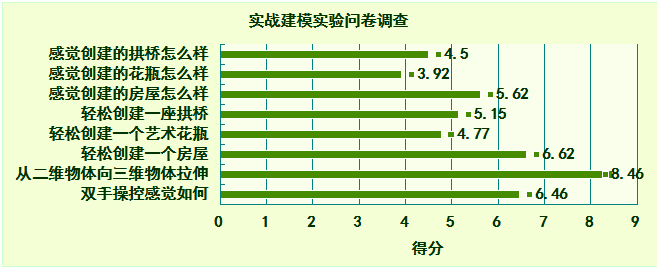
\includegraphics[width=0.8\textwidth]{chap6/eva-question-formal}
  \bicaption[fig:spcItrc:formal]{建模问卷调查}{建模问卷调查}{Fig.}{Formal experiment questionnaire}
\end{figure}

开始之前照例向实验者阐述了实验过程中要创建的三个模型,并且将模型的特性和本文系统的特性都分别予以了阐述,帮助实验者更好地理解本文系统与实验。从图\ref{fig:spcItrc:formal}中可以看到实验者对与三个模型创建的反馈。分数从0分到10分由低到高表示负面到正面的感受。首先我们可以看到拉伸手势的分数很高。每次用户创建一个三维模型都需要使用拉伸手势,也因此对于该手势的练习次数很多。同理可知对于绘制手势实验者也是较为熟悉。
%图\ref{fig:spcItrc:model}展示了部分实验者创建的模型,可以看到基本房屋的构造非常明晰,艺术花瓶的效果在变化的半径上略有体现,拱桥的弧度一样清晰可见,虽然不够大,但也是一个不错的开始。

对于三种模型的创建,我们结合用户在图\ref{fig:spcItrc:formal}的反馈中进一步分析。第一个模型是基本房屋,实验者只需要使用绘制之手(也就是惯用手)来完成该实验。大部分实验者在实验进行中要求进行多次,因为他们希望创建出不同形状的有趣的房子。其中一名实验者,没有任何使用虚拟现实或增强现实的设备经验,一共进行了四次最终绘制成功。无论如何实验者尝试建模的次数始终很小,同样表明本文系统提供的这套方法简单易上手。当实验者在创建房屋时,观察到实验者对与绘制手势的使用非常平滑自然且选择想要的控制点比在基本操控实验\ref{exp:cp}中要迅速很多。

图\ref{fig:spcItrc:time}显示了用户在创建房屋时的时间统计,观察可得时间的跨度并不大且实验者所需的时间均是一个较小的数值(ET)。
其中有一名实验者花费了接近三分钟去创建一个基本房屋,他觉得选中合适的点并拉伸略有困难,原因是他的手指总是在Leap Motion的检测范围之外。
很自然用户在不熟悉的设备下可能会导致预料之外的结果。
虽然我们在本文系统中提供了用户骨骼相关的提示帮助用户更好地完成建模,他们依旧需要一点时间来熟悉ARGlasses。
诚然这个基本房屋的模型非常简单,实验者不需要花费很多时间去创作,但当用户完成创建时,他们纷纷表示直接利用双手进行建模感受很不一样。
这就是徒手创作的魅力所在。并且从图\ref{fig:spcItrc:formal}中可以得知用户觉得创作房屋很轻松且对自己构建的房屋也比较满意。

\begin{figure}[!htp]
  \centering
  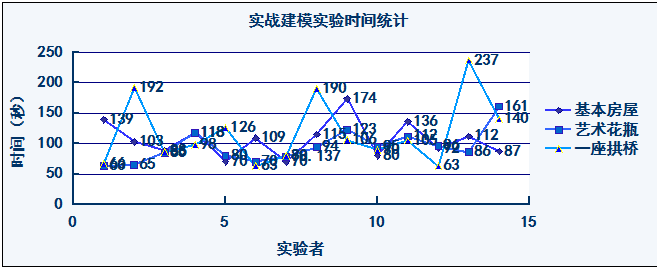
\includegraphics[width=0.9\textwidth]{chap6/eva-time}
  \bicaption[fig:spcItrc:time]{建模时间统计}{建模时间统计}{Fig.}{Time consumption on creating}
\end{figure}

第二个模型是艺术花瓶,其拥有用户自定义的半径变化。当实验者听说要创建一个婀娜多姿的花瓶时纷纷表示不可信、太复杂了。
而当我们解释了放缩工具的使用方法和两手之间的协作模式后,便表示制作这样一个花瓶也是可行且合理的。
从结果来看,实验者所需要尝试的次数比一个基本的房屋要多,最多的是五次。
实验者们的时间分布如图\ref{fig:spcItrc:time}所示(ET)。
实验者中最迅速的仅用一分钟完成创建任务,花费三分钟左右的实验者表示了双手协作的不适应。在空中悬停双手并完成不同任务使他们有些紧张。
而在练习了一两次后便适应很多,就像日常生活中左右手通常都负责不一样的任务一般。

图\ref{fig:spcItrc:formal}中我们可以看到对于花瓶模型的分数比基本房屋要低。
当然,花瓶的创建比房屋要更复杂,而且这也是首次实验者们使用双手协作来完成建模任务,而双手协作的分数为6.25,依然是一个尚可接受的评分。
在花瓶实验中我们要求实验者从旋转工具切换到放缩工具,有几次实验者忘记切换手势要转两圈因而切换失败,当然在我们提示或者他自行回想起来之后,实验者便可成功完成该项动作。
除此之外,部分实验者在创建过程中将模型沿自由虚拟网格平面的两个法向拉伸,于是创建除了非常不规则的物体,虽然并不是所需的创作目标,但这也让他们体会到了操控之手和绘制之手的结合。

第三个模型是拱桥。这个模型结合了旋转操控和绘制过程。
类似的,实验者最开始也表示无法绘制拱桥这样不规则的弯曲物体,而当我们仔细描述了本文系统支持的旋转工具后他们便跃跃欲试。
令人惊喜的是,实验者们的尝试次数反而没有创建花瓶时那么多。
平均次数约为2次。实验者在这个实验中表现得更为熟练,在拉伸桥墩时,实验者开始旋转以坐标轴为代理的旋转工具,尽管开始有些不适应,但在理解旋转的执行逻辑后,实验者便能照自己所想对自由虚拟网格平面进行旋转操控,继而进行旋转建模。

在图\ref{fig:spcItrc:time}中可以看到实验者需要约1分钟创建拱桥(ET)。
创建完后实验者表示这个徒手三维建模方法很有意思。
而在问卷调查中可以看到拱桥的得分比花瓶更高。
当时用户已经比创建花瓶是更熟悉工具的调用和双手协作的模式。
同样双手协作的得分也表明了职责分离这一设计的可行性。
\begin{table}[!htp]
  \centering
  \begin{minipage}[!htp]{0.6\textwidth}
  \captionstyle{\centering}
  \centering
	\bicaption[tab:exp:3dmax]{初学者使用Autodesk 3ds Max完成相同模型创建的的时间统计}{初学者使用Autodesk 3ds Max完成相同模型创建的的时间统计}{Table}{Time consumption for a pilot to create same models in Autodesk 3ds Max}
	\begin{tabular}{@{}cccc@{}} \toprule
    实验内容 & 实验1/秒 & 实验2/秒 & 实验3/秒 \\
	\midrule
    所需时间 & 57 & 61 & 51 \\
	\bottomrule
	\end{tabular}
   \end{minipage}
\end{table}
在完成所有实验后我们向实验者询问混合现实眼镜佩戴的舒适感,没有人表示不适,而对虚拟现实或增强现实设备较熟悉的用户在实验中学习得更快,当然没有该经验的实验者也一样完成了实验。
除此之外我们邀请一个有专业建模经验的志愿者教授一位初学实验者使用Autodesk 3ds Max进行相同模型的设计,其所花费时间如表\ref{tab:exp:3dmax}所示,观察可得时间花费相去不远。

\subsection{设计原则的定性分析}

\subsubsection{保持由右及左}
%\item 保持由右及左\hfill\\
本文所设计的系统中用户使用惯用手进行更细致的建模工作,使用非惯用手发布指令。在整个实验完成后,从实验者对于双手交互建模的评分中观察可得,实验者肯定该设计的以及适应在混合现实眼镜下使用此类交互方式。
\subsubsection{对称的移动规模}
%\item 对称的移动规模 \hfill\\
本文所设计的系统依旧安排用户使用惯用手完成更频繁的工作,实验进行中可以看到实验者更多地使用惯用手来调整自己的模型。同时我们并没有特意安排不同的工作空间给双手,特别是给非惯用手更大的工作空间,而在建模实验中实验者并没有对控制旋转工具或放缩工具的空间设定表示不满,也由此肯定了我们的这项决定。
\subsubsection{右手先行}
%\item[右手先行]\hfill\\
本文所设计的系统先让用户使用惯用手进行整个环境的初始化,初始化完成后,自由虚拟网格平面跃然眼前用户即可立刻开始点的绘制与模型创作,两个阶段近乎无缝衔接,同样也保证了用户的惯用手在工作空间内。若是使用左手进行初始化,势必会遇到右手没有完全找到工作空间或者只是纯粹的多做了一个动作这两种情况。因而在本应用环境下采用右手先行非常合理。
\subsubsection{自由虚拟网格平面}
%\item[自由虚拟网格平面]\hfill\\
自由虚拟网格平面的设定是为了保证用户的自由度且优化用户的绘制效果。用户所创建的各种各样的房屋、花瓶和拱桥已经验证了其自由度的保持,同时如基本操控实验中提到的绘制正方形这类规范绘图,用户一样可以轻松完成。也由此可见自由虚拟网格平面可以帮助用户既发挥自己的特性又规避自身绘制能力不足地进行模型创建。
\subsubsection{职责分离的双手}
%\item[职责分离的双手]\hfill\\
最后一个部分是职责分离的设计。通过职责分离帮助用户在建模过程中无缝切换状态。开始时用户习惯于放下右手抬起左手进行操作,反之亦然。而在我们提醒后便可以同时进行拉伸建模步骤和切换工具步骤。并且对这样的无缝建模过程可以迅速适应。
同时由于自由虚拟网格平面的存在,成功将整个空间划分为工作空间与非工作空间,因而用户没有出现过任何误操作行为干扰到当前的建模过程。
%\end{description}

\section{本章小结}
本章对本文所设计系统的所有设计与实现进行了详实的评估。
首先是对于混合现实眼镜下的三维菜单与三维操控,通过对每个操作设计用户实验进行可行性评估,而在该次实验中发现了设备上的缺陷,和一些显示上的不足,因而又增加了一些辅助设计。接着对设计的三种菜单布局进行偏好分析,设计了相同的实验内容来比较不同菜单的操作感受,对于通常任务时,喜好屏幕固定式菜单和手掌召唤式菜单的各有些许,对于菜单的选择反映了实验者思考问题的着重点的不同;而对于批处理任务时,几乎所有实验者都选择了手掌召唤式菜单。
接着对辅助设计与单双手的操控进行了易用性评估。
分别对每一项,顶置提示板、骨骼小球和头部约束进行各自的实验与分析,从用户选择保留与否与启动辅助设计与否的时间差对这些辅助设计的易用性进行评估。
同时为单手和双手操控设计了一样的实验,控制变量让用户感受两种方式的操控,并选择偏好的那种。
显然单双手的比较还有很多其他的领域可以探索,这里仅仅在效率和操作感上进行讨论。
接着对空间设计的基本操控进行评估,观察用户在基本的绘制、拉伸、旋转和放缩操控上是否有困难,最后让用户进行完整的多个模型创建,结合操控之手和绘制之手进行双手建模体验。
通过用户的主观反馈和时间等数据的客观记录,评判可得该徒手三维建模方法的实用性。其后针对每个空间设计上采用的设计原则和提出的方法分别予以分析,完成了本文系统的所有实验与评估。